\section{Problem: Where the Value of Cooperation Is Lost}
\label{sec:problem}

\subsection{Setting}
\label{sec:setting}
An ego vehicle $e$ and a roadside unit $i$ each run a LiDAR detector.
At decision time $t$ the ego detector outputs boxes $\mathcal B_e(t)=\{(\mathbf b_k,s_k)\}$, and the roadside unit broadcasts messages $m_\tau=(\mathcal B_i(\tau),\tau)$ with its detections at capture time $\tau$.
Under the \emph{strict arrival protocol} the receiver may use only messages with $\tau\le t-d$ for a latency budget $d$; frames without an admissible message are still evaluated.
Remote boxes are mapped into the ego frame with the poses available online---the vehicle localisation $\mathbf T_{w\leftarrow e}(t)$ and the roadside calibration $\mathbf T_{w\leftarrow i}$---so that $\mathbf T_{e\leftarrow i}(t)=\mathbf T_{w\leftarrow e}(t)^{-1}\mathbf T_{w\leftarrow i}$.
No ground truth, future frame or per-pair calibration offset is used at inference.
The task is to detect vehicles in the ego frame at time $t$.

\subsection{Geometry, not latency, dominates}
\label{sec:geometry}
\Cref{fig:latency} shows \apseven on the 21 validation sequences against the latency budget (exact numbers in \cref{tab:main}).
Three observations frame the rest of the paper.
\emph{(i) Cooperation barely helps as practised.}
Late fusion of the released TraF-Align~\cite{song2025trafalign} boxes with online poses improves \apseven over the ego detector by 1.0 point, to 63.18 on average, and the official late-fusion baselines and three intermediate-fusion models stay between 61.1 and 63.0.
\emph{(ii) The value is recoverable.}
Placing the same remote boxes with the dataset's annotation-assisted offset, one planar translation per frame, gives 69.52 \apseven: one translation per message adds 6.3 points over online poses and turns a 1.0-point gain of cooperation into a 7.4-point gain.
\emph{(iii) Latency costs little in comparison.}
With good geometry, \apseven drops by 2.3 points from 0 to 400\,ms with the dataset offset (70.59 to 68.33) and by 1.7 points with \method (67.37 to 65.72), well below the geometric gap.

\begin{figure}[t]
  \centering
  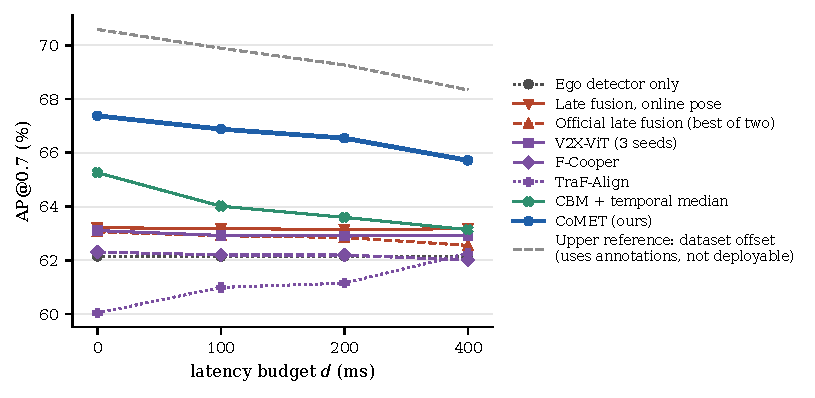
\includegraphics[width=0.78\linewidth]{fig/latency.pdf}
  \caption{\textbf{\apseven against the latency budget on V2X-Seq validation.} Intermediate fusion and late fusion with online poses stay close to the ego detector. \method recovers over half of the gap to the upper reference that places the boxes with the dataset's annotation-assisted offset (dashed gray, not deployable). Values are means over three readout heads or three detector seeds; numbers in \cref{tab:main}.}
  \label{fig:latency}
\end{figure}

\subsection{A shared, persistent, sparsely observed error}
\label{sec:structure}
We model the centre of remote object $j$ after mapping to the ego frame as
\begin{equation}
  \tilde{\mathbf x}_j=\mathbf x_j-\boldsymbol\delta_t+\boldsymbol\epsilon_j ,
  \label{eq:model}
\end{equation}
where $\mathbf x_j$ is its true centre, $\boldsymbol\delta_t$ a planar correction shared by all objects of the message (the common mode) and $\boldsymbol\epsilon_j$ an object-specific error from detection noise and residual motion.
Such a shared term arises when the dominant error lies in the transform that maps the roadside frame into the ego frame---a residual calibration or localisation bias---which displaces every object of a message alike, whereas detection noise and uncompensated motion act on each object separately.
Three properties make this model useful.

\emph{Observable.}
For an object seen by both agents, the residual $\mathbf z=\mathbf x^{\text{ego}}-\tilde{\mathbf x}$ between the ego box and the projected remote box equals $\boldsymbol\delta_t$ plus noise, with no label involved.
The same $\boldsymbol\delta_t$ then corrects the remote objects that the ego vehicle cannot see.

\emph{Sparse per message.}
Using all ego detections and mutual-nearest-neighbour matching within 2.5\,m (\cref{sec:method}), a validation message contains 2.96 anchors on average at $d=0$ (2.73 at 400\,ms), and 38.2\% of messages contain none; messages that do contain anchors hold 4.79 of them.
Estimating $\boldsymbol\delta_t$ from the current message alone is therefore often impossible and, when possible, noisy: against a smoothed reference built from the dataset offsets (only used for analysis), the per-message estimate has a radial RMSE of 0.48\,m at $d=0$ and 0.61\,m at $d=400$\,ms on messages with anchors, and misses by more than 1\,m on 4\% and 9\% of them; moving anchors increasingly mix the pose error with uncompensated motion as the message ages.
The tracked estimate of \method has 0.41\,m RMSE at both budgets and misses by more than 1\,m on 2\%.

\emph{Persistent.}
Within a sequence the offset changes slowly compared with the 10\,Hz message rate (\cref{fig:trajectory}).
The common-mode error should therefore be \emph{tracked} over the message stream rather than re-estimated in every frame.

\begin{figure}[t]
  \centering
  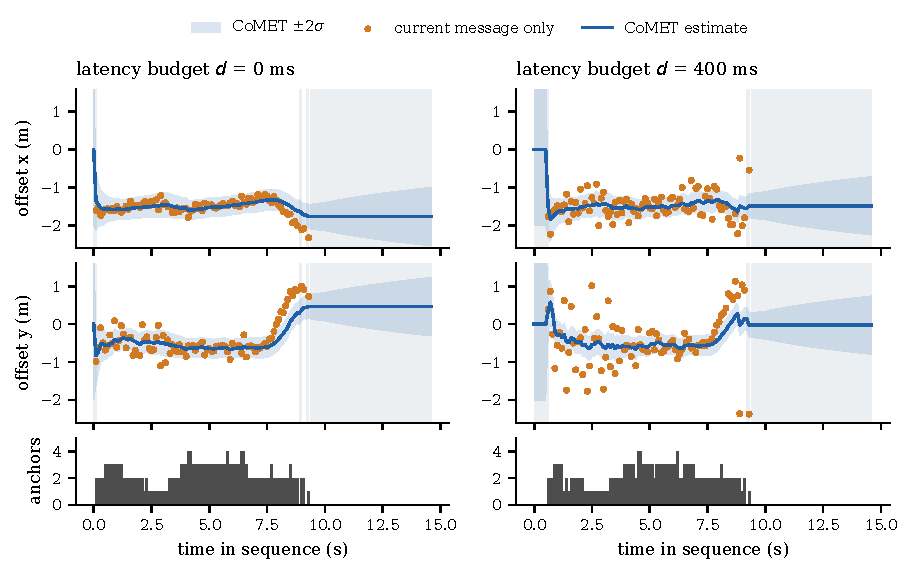
\includegraphics[width=\linewidth]{fig/trajectory.pdf}
  \caption{\textbf{One validation stream (sequence 0007) at two latency budgets.} Orange: offset estimated from the anchors of the current message only (shown only when the message has anchors). Blue: the \method estimate with its $\pm2\sigma$ band; gray bands mark messages without anchors. Bottom: number of anchors per message. The per-message estimate is noisy and disappears when anchors are absent (after about 9\,s); the tracked estimate is stable, follows the change in $y$ around 8\,s, and keeps the last estimate with growing uncertainty when anchors vanish. At 400\,ms the per-message estimate is noticeably noisier.}
  \label{fig:trajectory}
\end{figure}

\subsection{The benchmark's reference offset}
\label{sec:audit}
V2X-Seq provides a per-pair \texttt{system\_error\_offset}, a planar translation estimated offline for each vehicle--roadside frame pair.
Prior work trains and evaluates with these offsets as the calibrated relative pose.
Because they also define what ``correct geometry'' means in \cref{sec:geometry}, we audit them directly against the raw annotations of all 67 training and validation sequences (\cref{tab:census}, \cref{fig:audit}; details in \cref{app:audit}).

\begin{table}[t]
  \centering
  \caption{\textbf{Census of the dataset offset per split.} Messages with an offset of exactly $(0,0)$; among them, those that still contain a co-labelled object; non-zero messages without a co-labelled object; and non-zero messages with at least one axis on the search bound ($-1.1$ or $+0.66$\,m), as a fraction of non-zero messages.}
  \label{tab:census}
  \small
  \begin{tabular}{lrrrrr}
    \toprule
    Split & Messages & Exactly zero & \makecell{Zero with\\co-labelled obj.} & \makecell{Non-zero without\\co-labelled obj.} & \makecell{Non-zero\\on a bound} \\
    \midrule
    \tabinput{tables/census.tex}
    \bottomrule
  \end{tabular}
\end{table}

\paragraph{A placeholder.}
The offset is exactly zero on 21.8--28.0\% of the messages of each split.
Outside the calibration split, no zero message contains a co-labelled object (an object annotated by both agents), and only 10--16 of the messages without a co-labelled object have a non-zero offset.
Zero is therefore a placeholder for ``could not be estimated'', not a measurement of zero error.
The calibration split contains 35 zero messages that do have a co-labelled object; there the roadside and vehicle labels of that object differ by 1.22\,m (median), so the placeholder is not a statement that the error vanished.

\paragraph{The offset is inside the ground truth.}
For roadside-only objects, the cooperative ground truth equals the public projection of the roadside label plus the offset, with a residual of about $4\times10^{-7}$\,m in both the zero and the non-zero case.
On placeholder messages the ground truth of roadside-only objects is therefore the \emph{uncorrected} projection.
A method that estimates the true shift on such a message moves its boxes away from this ground truth and is penalised; a method that does nothing is rewarded.

\paragraph{A bounded discrete search.}
The non-zero offsets take only 26 distinct values per axis including zero, in five groups with a step of 0.04\,m, bounded by $-1.1$ and $+0.66$\,m (\cref{fig:audit}a,b).
At least one axis sits on a bound for 44.6\% of the non-zero validation messages (77.7\% in the calibration split).
On the bound the co-labelled objects of the same frame are typically displaced further: on the $x=-1.1$ bound (2,413 frames with at least three co-labelled objects) their median displacement is $-1.37$\,m and 91\% of the frames lie beyond the bound; on the $y=+0.66$ bound the median is $+0.93$\,m.
Across frames with at least three co-labelled objects, displacements larger than 1.5\,m occur in 19.6\% of frames but official offsets in only 1.1\%.
We infer the search structure from the values alone; the generating procedure is not documented.

\begin{figure}[t]
  \centering
  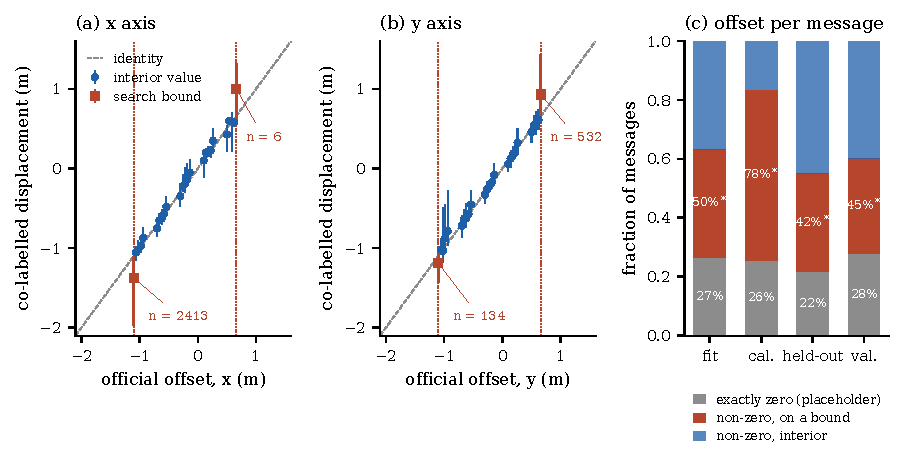
\includegraphics[width=\linewidth]{fig/offset_audit.pdf}
  \caption{\textbf{The dataset offset is a bounded discrete search with a zero placeholder.} (a,b) For each value the offset takes on an axis, the median and 10--90\% range of the displacement of co-labelled objects in the same frame (frames with at least three co-labelled objects, all splits). Interior values follow the diagonal; on the bounds (red) the objects are displaced further than the offset. (c) Per split, the share of messages with an exactly zero offset (gray, percentage of all messages), a non-zero offset on a bound (red; the percentage marked $^*$ is relative to non-zero messages), and an interior non-zero offset (blue).}
  \label{fig:audit}
\end{figure}

\paragraph{Consequences for evaluation.}
The dataset offset is a label-consistent reference, not an oracle: it is zero where it could not be estimated and clipped where the error is large, and the ground truth inherits both properties.
We keep the official ground truth for all primary results and add two complementary readings (\cref{sec:protocol}): results split into label-defined populations (all, exactly zero, with co-labelled objects), and two auxiliary references that re-register roadside-only ground truth on placeholder frames (by interpolating the non-zero offsets of the same sequence) or on all frames with at least three co-labelled objects (by their median displacement).
Neither auxiliary reference is physical truth; they show which conclusions depend on the label artefacts.
